%%%%%%%%%%%%%%%%%%%%%%%%%%%%%%%%%%%%%%%%%
% fphw Assignment
% LaTeX Template
% Version 1.0 (27/04/2019)
%
% This template originates from:
% https://www.LaTeXTemplates.com
%
% Authors:
% Class by Felipe Portales-Oliva (f.portales.oliva@gmail.com) with template 
% content and modifications by Vel (vel@LaTeXTemplates.com)
%
% Template (this file) License:
% CC BY-NC-SA 3.0 (http://creativecommons.org/licenses/by-nc-sa/3.0/)
%
%%%%%%%%%%%%%%%%%%%%%%%%%%%%%%%%%%%%%%%%%

%----------------------------------------------------------------------------------------
%	PACKAGES AND OTHER DOCUMENT CONFIGURATIONS
%----------------------------------------------------------------------------------------

\documentclass[
	12pt, % Default font size, values between 10pt-12pt are allowed
	%letterpaper, % Uncomment for US letter paper size
	%spanish, % Uncomment for Spanish
]{fphw}

% Template-specific packages
\usepackage[utf8]{inputenc} % Required for inputting international characters
\usepackage[T1]{fontenc} % Output font encoding for international characters
%\usepackage{mathpazo} % Use the Palatino font

\usepackage{graphicx} % Required for including images

\usepackage{booktabs} % Required for better horizontal rules in tables

\usepackage{listings} % Required for insertion of code
\usepackage{mathtools}
\usepackage{nccmath}
\usepackage{amsmath}
\usepackage{enumerate} % To modify the enumerate environment
\usepackage{graphicx}
\usepackage{caption}
\usepackage{float}
\usepackage{subcaption}
\newtheorem{theorem}{Theorem}
\newtheorem{corollary}{Corollary}[theorem]
\newtheorem{definition}{Definition}
%----------------------------------------------------------------------------------------
%	ASSIGNMENT INFORMATION
%----------------------------------------------------------------------------------------

\title{Homework \#1} % Assignment title

\author{Antonio Albanese, 282043} % Student name

\date{November 2021} % Due date

\institute{Politecnico di Torino} % Institute or school name

\class{Networks dynamics and Learning} % Course or class name

\professor{Dr. Albert Einstein} % Professor or teacher in charge of the assignment

%----------------------------------------------------------------------------------------

\begin{document}

\maketitle % Output the assignment title, created automatically using the information in the custom commands above

%----------------------------------------------------------------------------------------
%	ASSIGNMENT CONTENT
%----------------------------------------------------------------------------------------
\emph{In this homework I exchanged ideas and compared results with my colleague Nedescu Ionut Cosmin.}

\vspace{10pt}

\emph{Please note that the report seems to be too long because text of the assignment was also reported to have simpler references to pictures and equations. Thank you.}
\section*{Exercise 1}


Consider unitary o-d network (i.e., integer whose integer units cannot be
split) on the graph $\mathcal{G} = (\mathcal{V}; \mathcal{E})$ in Figure \ref{fig:givenGraphEx1}, and assume that each link l has integer capacity $C_l$.
\begin{figure}[H]
    \centering
	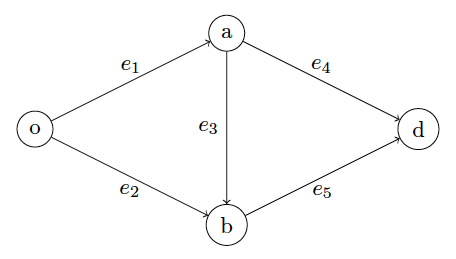
\includegraphics[width=0.5\columnwidth]{graphEx1.png} % Example image
	\caption{}
	\label{fig:givenGraphEx1}
\end{figure}
\begin{enumerate}[(a\normalfont)] % Sub-questions styled as italic letters
	\item What is infimum of the total capacity that needs to be removed for no feasible unitary flows from $o$ to $d$ to exist?
	\item Assume that the link capacities are
	    \begin{equation}\label{eq:capacitiesEq}
	        C_1 = C_4 = 3, \hspace{20pt} C_2 = C_3 = C_5 = 2.
	   \end{equation}
	    Where should 1 unit of additional capacity be allocated in order to maximize the feasible throughput from o to d? What is the maximal throughput?
	\item Consider link capacities (\ref{eq:capacitiesEq}). Where should 2 units of additional capacity be allocated in order to maximize the feasible throughput from $o$ to $d$? Compute all the optimal capacity allocations for this case and the optimal throughput.
	\item Consider link capacities (\ref{eq:capacitiesEq}). Where should 4 units of additional capacity be allocated in order to maximize the feasible throughput from $o$ to $d$? Compute all the optimal capacity allocations for this case. Among the optimal allocations, select the allocation that maximizes the sum of the cut capacities.
\end{enumerate}

%------------------------------------------------

\subsection*{Answer}%Answer 1
\begin{enumerate}[{\bfseries (a)}]
    \item To answer this question we need to start from three concepts:
    \begin{definition}[Node-independent paths]
        Two $i-j$ paths are    \emph{node-independent} if they share no intermediate node.
    \end{definition}
    \begin{definition}[Link connectivity]
        The \emph{link-connectivity} $c_{link}(i,j)$ of a pair of nodes $(i, j)$ is the maximum number of \emph{link-independent} $i-j$ paths.
    \end{definition}
    \begin{theorem}[Menger's Theorem]
        The minimum number of links that have to be removed from a graph $\mathcal{G}$ in order for node $j$ not to be reachable from node $i$ equals $c_{link}(i, j)$.
    \end{theorem}
    
    In the given graph we have  $c_{link}(o,d) = 2$, meaning that we need to remove at least 2 links to have no feasible flow from $o$ to $d$. 
    
    The infimum of  the  total  capacity  that  needs  to  be  removed  for  no  feasible unitary flows from $o$ to $d$ to exist is 
    $$
        \mathbf{\min{\{(C_1+C_2), (C_1+C_5), (C_4+C_5), (C_1,C_3,C_5)\}}}
    $$
    
    
    \item First of all we can redraw the graph with the given capacities (\ref{eq:capacitiesEq}) (Figure \ref{fig:figEx1b}).
        
        \begin{figure}[H]
        \centering
        	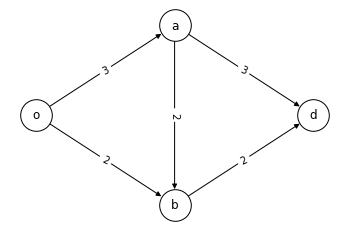
\includegraphics[width=0.5\columnwidth]{graph1-b.png} % Example image
        	\caption{Redrawn graph with explicit capacities assigned to links}
        	\label{fig:figEx1b}
        \end{figure}
        To answer this question we can use \emph{max-flow min-cut theorem}.
        First we need a couple of definitions.
        \begin{definition}[Maximum throughput]
            For a capacited multigraph $\mathcal{G} = (\mathcal{V}; \mathcal{E}; c)$ and two distinct nodes $o \neq d$ in $\mathcal{V}$, the maximum-flow problem is the constraint maximization problem
            $$
                \chi^*_{o,d} = \max_{\substack{\chi \geq 0\\ 0 \leq f \leq c\\ Bf = \chi(\delta^{(o)} - \delta^{(d)})}}\chi
            $$
            $\chi^*_{o,d}$ is the \emph{maximum throughput} from $o$ to $d$.
        \end{definition}
        \begin{definition}[Min-cut capacity]
            We fix a multigraph $\mathcal{G} = (\mathcal{V}; \mathcal{E}; c)$ and two distinct nodes $o \neq d$ in V. 
            The \textbf{min-cut capacity} of the network is the value
            $$
              c^*_{o,d} = \min_{\substack{\mathcal{U} \subseteq \mathcal{V}\\ o \in \mathcal{U}, d \notin \mathcal{U}}} c_{\mathcal{U}} 
            $$
        \end{definition}
        \begin{theorem}[Max-flow min-cut theorem]
            Consider a multigraph $\mathcal{G} = (\mathcal{V}; \mathcal{E}; c)$ with a capacity vector $c > 0$, and two distinct nodes $o \neq d$ in $\mathcal{V}$. Then, 
            $$
                \chi^*_{o,d} = c^*_{o,d}.
            $$
        \end{theorem}
        Theorem 2 tells us that the maximum throughput from $o$ to $d$ equals the min-cut capacity from $o$ to $d$.\\
        In the given graph we have the following cuts: 
        \begin{itemize}
            \item $U=\{o,b,a\},U^C=\{d\}$ -> $C_U = 5$
            \item $U=\{o,a\},U^C=\{b,d\}$ -> $C_U = 7$
            \item $U=\{o,b\},U^C=\{a,d\}$ -> $C_U = 5$
            \item $U=\{o\},U^C=\{a,b,d\}$ -> $C_U = 5$
        \end{itemize}
        
        The minimum cut capacity is 5 and there are three cuts, whit that capacity.
        \begin{itemize}
            \item cut $U=\{o,b,a\},U^C=\{d\}$,
                    \begin{equation}
                        C_U = c(b,d) + c(a,d)
                        \label{eq:eqCut1}
                    \end{equation}
            \item cut $U=\{o,b\},U^C=\{a,d\}$,
                    \begin{equation}
                        C_U = c(o,a) + c(b,d)
                        \label{eq:eqCut2}
                    \end{equation}
            \item cut $U=\{o\},U^C=\{a,b,d\}$,
                    \begin{equation}
                        C_U = c(o,a) + c(o,b)
                        \label{eq:eqCut3}
                    \end{equation} 
        \end{itemize}
        
        Independently on which of those links we apply one more unit of capacity the \textbf{max throughput can not be improved}.

        \item Starting from what we know in \textbf{(b)} and equations (\ref{eq:eqCut1}), (\ref{eq:eqCut2}) and (\ref{eq:eqCut3}) we can optimize the choice of links on which to add capacities with the aim to increase the max-flow.\\
        With a recursive function it was possible to calculate all the optimal capacity allocations finding three possibilities:
        \begin{itemize}
            \item Adding 1 unit to $(o,a)$ and 1 unit $(a,d)$
            \item Adding 1 unit to $(o,a)$ and 1 unit $(b,d)$
            \item Adding 1 unit to $(o,b)$ and 1 unit $(b,d)$
        \end{itemize}
        All solutions found give min-cut capacity equals to 6.\\ 
        For example we could choose the configuration 
        $$
        \begin{cases}
            c(a,b) = 2 \rightarrow c(a,b) = 2,\\
            c(a,d) = 3 \rightarrow c(a,d) = 3,\\
            \bf{c(b,d) = 2 \rightarrow c(b,d) = 4},\\
            c(o,a) = 3 \rightarrow c(o,a) = 3,\\
            \bf{c(o,b) = 2 \rightarrow c(o,b) = 4}
        \end{cases}
        $$
        with
        \begin{itemize}
            \item $U=\{o,b,a\},U^C=\{d\}$ -> $C_U = c(b,d) + c(a,d) = 6$
            \item $U=\{o,a\},U^C=\{b,d\}$ -> $C_U = 7$
            \item $U=\{o,b\},U^C=\{a,d\}$ -> $C_U = c(o,a) + c(b,d) = 6$
            \item $U=\{o\},U^C=\{a,b,d\}$ -> $C_U = c(o,a) + c(o,b) = 6$.
        \end{itemize}
        Again, following the \emph{max-flow min-cut theorem} we know that the \textbf{maximum throughput now is 6}. 
        
        \item This part is similar to \textbf{(c)} and with the same recursive function it was possible to calculate all the optimal capacity allocations, resulting in six different possibilities:
        \begin{enumerate}[1)]
            \item Adding 2 units to $(o,a)$ and 2 unit $(a,d)$ 
            \begin{itemize}
                \item $U=\{o,b,a\},U^C=\{d\}$ -> $C_U = 7$
                \item $U=\{o,a\},U^C=\{b,d\}$ -> $C_U = 9$
                \item $U=\{o,b\},U^C=\{a,d\}$ -> $C_U = 7$
                \item $U=\{o\},U^C=\{a,b,d\}$ -> $C_U = 7$.
            \end{itemize}
            \item Adding 2 units to $(o,a)$, 1 unit to $(a,d)$ and 1 unit to $(b,d)$ 
            \begin{itemize}
                \item $U=\{o,b,a\},U^C=\{d\}$ -> $C_U = 7$
                \item $U=\{o,a\},U^C=\{b,d\}$ -> $C_U = 8$
                \item $U=\{o,b\},U^C=\{a,d\}$ -> $C_U = 8$
                \item $U=\{o\},U^C=\{a,b,d\}$ -> $C_U = 7$.
            \end{itemize}
            \item Adding 2 units to $(o,a)$ and 2 units to $(b,d)$
            \begin{itemize}
                \item $U=\{o,b,a\},U^C=\{d\}$ -> $C_U = 7$
                \item $U=\{o,a\},U^C=\{b,d\}$ -> $C_U = 7$
                \item $U=\{o,b\},U^C=\{a,d\}$ -> $C_U = 9$
                \item $U=\{o\},U^C=\{a,b,d\}$ -> $C_U = 7$.
            \end{itemize}
            \item Adding 1 unit to $(o,a)$ and 1 unit to $(o,b)$, 1 unit to $(a,d)$ and 1 unit to $(b,d)$
            \begin{itemize}
                \item $U=\{o,b,a\},U^C=\{d\}$ -> $C_U = 7$
                \item $U=\{o,a\},U^C=\{b,d\}$ -> $C_U = 9$
                \item $U=\{o,b\},U^C=\{a,d\}$ -> $C_U = 7$
                \item $U=\{o\},U^C=\{a,b,d\}$ -> $C_U = 7$.
            \end{itemize}
            \item Adding 1 unit to $(o,a)$ and 1 unit to $(o,b)$ and 2 units to $(b,d)$
            \begin{itemize}
                \item $U=\{o,b,a\},U^C=\{d\}$ -> $C_U = 7$
                \item $U=\{o,a\},U^C=\{b,d\}$ -> $C_U = 9$
                \item $U=\{o,b\},U^C=\{a,d\}$ -> $C_U = 7$
                \item $U=\{o\},U^C=\{a,b,d\}$ -> $C_U = 7$.
            \end{itemize}
            \item Adding 2 units to $(o,b)$ and 2 units to $(b,d)$
            \begin{itemize}
                \item $U=\{o,b,a\},U^C=\{d\}$ -> $C_U = 7$
                \item $U=\{o,a\},U^C=\{b,d\}$ -> $C_U = 9$
                \item $U=\{o,b\},U^C=\{a,d\}$ -> $C_U = 7$
                \item $U=\{o\},U^C=\{a,b,d\}$ -> $C_U = 7$.
            \end{itemize}
        \end{enumerate}
        In all the configurations shown the cut capacities sum up to 30, so we can choose any of them. 
            
            For example choosing option 4: 
            $$
            \begin{cases}
                c(a,b) = 2 \rightarrow c(a,b) = 2,\\
                \bf{c(a,d) = 3 \rightarrow c(a,d) = 4},\\
                \bf{c(b,d) = 2 \rightarrow c(b,d) = 3},\\
                \bf{c(o,a) = 3 \rightarrow c(o,a) = 4},\\
                \bf{c(o,b) = 2 \rightarrow c(o,b) = 3}
            \end{cases}
            $$
            
            \textbf{The sum of cuts capacities is 30}.
            And following the \emph{max-flow min-cut theorem} \textbf{the maximum throughput is 7}.
\end{enumerate}


%----------------------------------------------------------------------------------------

\section*{Exercise 2}

	Consider the following problem. There are a set of people $(p_1, p_2, p_3, p_4)$ and a set of books $(b_1, b_2, b_3, b_4)$. Each person is interested in a subset of books, specifically 
	\begin{equation}
	    p_1 \rightarrow (b_1, b_2),\hspace{15pt} p_2 \rightarrow (b_2, b_3),\hspace{15pt} p_3 \rightarrow (b_1, b_4),\hspace{15pt} p_4 \rightarrow (b_1, b_2, b_4)
	    \label{eq:eqRelEx2}
	\end{equation}
	
	
	\begin{enumerate}[(a\normalfont)] % Sub-questions styled as italic letters
		\item Represent the interest pattern by using a simple bipartite graph.
		\item Exploit max-flow problems to establish whether there exists a perfect matching that assigns to every person a book of interest. If a perfect matching exists, find at least a perfect matching.
		\item Assume now that there are multiple copies of book, specifically the distribution of the number of copies is (2; 3; 2; 2), and there is no constraint on the number of books that each person can take. The only constraint is that each person can not take more copies of the same book. Use the analogy with max-flow problems to establish how many books of interest can be assigned in total.
		\item Starting from point (c), suppose that the library can sell a copy of a book and buy a copy of another book. Which books should be sold and bought to maximize the number of assigned books?
	\end{enumerate}

%------------------------------------------------

\subsection*{Answer}%Answer 2

\begin{enumerate}[{\bfseries (a)}]
    \item 
    \begin{definition}[Bipartite graph]
    A simple graph $\mathcal{G} = (\mathcal{V}, \mathcal{E}, W)$ is bipartite if and only if every circuit in $\mathcal{G}$ has even length.
    \end{definition}
    In other words a bipartite graph is a graph whose nodes can be divided into two disjoint and independent sets $\mathcal{V}^{(1)}$ and $\mathcal{V}^{(2)}$ such that every edge connects a node in $\mathcal{V}^{(1)}$ to at least one in $\mathcal{V}^{(2)}$, and there are no edges between nodes of the same set.\\
    Given the relations in (\ref{eq:eqRelEx2}) we can draw a bipartite graph as in Figure \ref{fig:figEx2a}.
    \begin{figure}[H]
        \centering
    	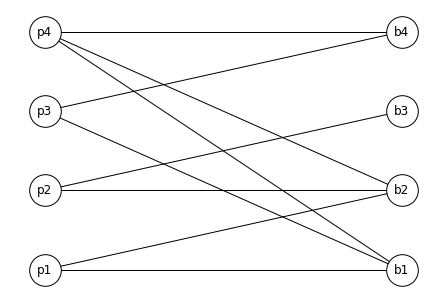
\includegraphics[width=0.5\columnwidth]{graph2a.png} % Example image
    	\caption{Relations in (\ref{eq:eqRelEx2})} represented as simple bipartite graph.
        \label{fig:figEx2a}
    \end{figure}
    \item 
    \begin{definition}[Matching]
        A matching or independent link set in an undirected graph $\mathcal{G} = (\mathcal{V}, \mathcal{E}, W)$ without self loops is a subset of links $\mathcal{M} \in \mathcal{E}$ that have no node in common.
    \end{definition}
    \begin{definition}[Perfect matching]
        A matching is \textbf{perfect} (sometimes also called complete) if all nodes are matched.
    \end{definition}
    \vspace{5pt}
    To exploit the max-flow problems to find a perfect matching (so to use the Hall's Marriage Theorem) we need to build the corresponding capacited directed multigraph of the given graph adding to the graph a source node $o$ and a sink node $d$, and giving each link capacity 1 (Figure \ref{fig:graph2B(a)}).\\ 
    \begin{figure}[H]
    \centering
        \begin{subfigure}{.5\textwidth}
            \centering
            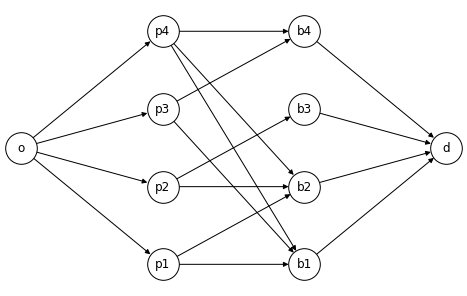
\includegraphics[width=1\linewidth]{2b(1).png}
            \caption{Graph redrawn with added nodes and directed edges}
            \label{fig:graph2B(a)}
        \end{subfigure}%
        \begin{subfigure}{.5\textwidth}
            \centering
            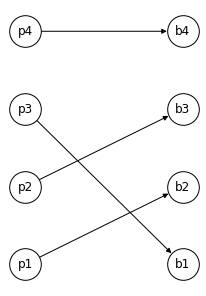
\includegraphics[width=0.5\linewidth]{2b.png}
            \caption{The perfect matching found}
            \label{fig:graph2B(b)}
        \end{subfigure}
        \caption{}
        \label{fig:figEx2b}
    \end{figure}
    \textbf{Using the max-flow algorithm it was possible to find a perfect matching}, depicted in Figure \ref{fig:graph2B(b)}. 
    
    \item We can start from the capacited multigraph found in \textbf{(b)}. 
    We know that people have multiple preferences of books, and this time we can assign more copies of a single book, but not at the same person.
    We can modify the graph in Figure \ref{fig:graph2B(a)} obtaining the graph in Figure \ref{fig:graph2C(a)}, in this way:
    \begin{itemize}
        \item Set capacity of edges $(o, p_i) = w_{p_i}$, where $w_{p_i}$ is the \emph{out degree} of the node $p_i$, meaning the number of different preferences of $p_i$
        \item Set capacity of existing edges $(p_i, b_j)$ to $1$, meaning that only one copy of the same book can be assigned to the same person
        \item Set capacity of edges $(b_j, d)$ equals to the number of different copies of each book that can be assigned.
    \end{itemize}
    \begin{figure}[H]
    \centering
        \begin{subfigure}{.5\textwidth}
            \centering
            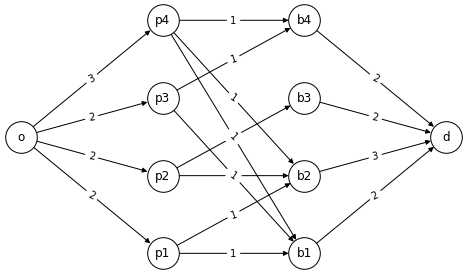
\includegraphics[width=1\linewidth]{2C(a).png}
            \caption{Graph redrawn with updated capacities}
            \label{fig:graph2C(a)}
        \end{subfigure}%
        \begin{subfigure}{.5\textwidth}
            \centering
            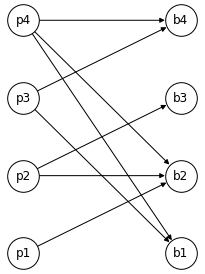
\includegraphics[width=0.5\linewidth]{2C(b).png}
            \caption{The best assignment found}
            \label{fig:graph2C(b)}
        \end{subfigure}
        \caption{}
        \label{fig:figEx2c}
    \end{figure}
    In this way \textbf{the maximum number of copies that can be assigned equals the max-flow between $\mathbf{o}$ and $\mathbf{d}$} that is $\mathbf{8}$. (Figure \ref{fig:graph2C(b)})
    
    \item The goal at this point is to maximize the number of assigned books, in other words try to satisfy all people preferences.\\ 
    Because of the manner in which we built the capacited graph (Figure \ref{fig:graph2C(a)}) in \textbf{(c)} we know that $w_{p_i}$, the \emph{out degree} of each node $p_i$, is the number of different books choosen by $p_i$, and it flows directly that $w^-_{b_j}$, the \emph{in degree} of each node $b_j$ is the total number of request for each book, while $w_{b_j}$, the \emph{out degree} of each node $b_j$, is the total number of copies that can be assigned for each book. 
    
    To miximize the number of assigned book and satisfy all users, we need that $w^-_{b_j} = w_{b_j}$.
    \begin{itemize}
        \item $b_1 \rightarrow w^-_{b_1} = 3, \hspace{10pt} w_{b_1} = 2 \Rightarrow $ \textbf{buy 1 copy of $b_1$}
        \item $b_2 \rightarrow w^-_{b_2} = 3, \hspace{10pt} w_{b_2} = 3$
        \item $b_3 \rightarrow w^-_{b_3} = 1, \hspace{10pt} w_{b_3} = 2 \Rightarrow$ \textbf{sell 1 copy of $b_3$}
        \item $b_4 \rightarrow w^-_{b_4} = 2, \hspace{10pt} w_{b_j} = 2$
    \end{itemize}
    In this way we can assign \textbf{9} copies in total. 
    
\end{enumerate}

%----------------------------------------------------------------------------------------

\section*{Exercise 3}


We are given the highway network in Los Angeles, see Figure 2. To simplify the problem, an approximate highway map is given in Figure 3, covering part of the real highway network. The node-link incidence matrix B, for this traffic network is given in the file \emph{traffic.mat}.
The rows of B are associated with the nodes of the network and the columns of B with the links.
The $i$-th column of B has 1 in the row corresponding to the tail node of link $e_i$ and (-1) in the row corresponding to the head node of link $e_i$. Each node represents an intersection between highways (and some of the area around).
\vspace{10pt}

Each link $e_i \in \{e_1, . . . ,e_{28}\}$, has a maximum-flow capacity $C_{e_i}$ . The capacities are given as a vector $C_e$ in the file \emph{capacities.mat}. Furthermore, each link has a minimum travelling time,
which the drivers experience when the road is empty. In the same manner as for the capacities, the minimum travelling times are given as a vector $l_e$ in the file \emph{traveltime.mat}. These values are simply retrieved by dividing the length of the highway segment with the assumed speed limit 60 miles/hour.


\begin{figure}[H]
	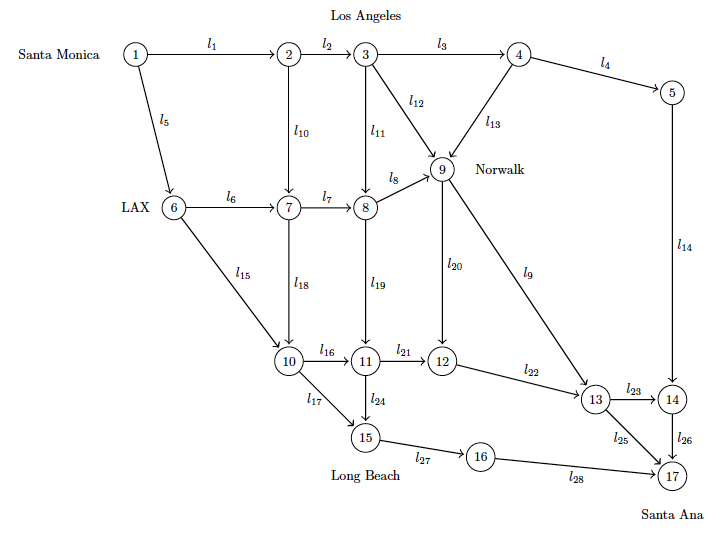
\includegraphics[width=0.8\columnwidth]{graphEx2.png} % Example image
	\caption{Some possible paths from Santa Monica (node 1) to Santa Ana (node 17).}
	\label{fig:graphEx3}
\end{figure}

For each link, we introduce the delay function
    \begin{equation}\label{eq:delayEq}
        d_e(f_e) = \frac{l_e}{1 - f_e/C_e}, \hspace{10pt} 0 \leq f_e \leq C_e
    \end{equation}
For $f_e \geq C_e$, the value of $d_e(f_e)$ is considered as $+\infty$.
\smallskip
\begin{enumerate}[(a\normalfont)] % Sub-questions styled as italic letters
		\item Find the shortest path between node 1 and 17. This is equivalent to the fastest path (path with shortest traveling time) in an empty network.
		\item Find the maximum-flow between node 1 and 17.
		\item Given the flow vector in \emph{flow.mat}, compute the external inflow $\nu$ satisfying $B f = \nu$.\\
		In the following, we assume that the exogenous inflow is zero in all the nodes except for node 1, for which $\nu_1$ has the same value computed in the point (c), and node 17, for which $\nu_{17} = - \nu_1$.
		\item Find the social optimum $f^*$ with respect to the delays on the different links $d_e(f_e)$. For this, minimize the cost function
		$$ 
		    \sum_{e \in \mathcal{E}} f_e d_e(f_e) = \sum_{e \in \mathcal{E}} \frac{f_e l_e}{1 - f_e/C_e} = \sum_{e \in \mathcal{E}} \left( \frac{l_e C_e}{1 - f_e/C_e} - l_e C_e \right)
		$$
		subject to the flow constraints.
		\item 
		    \begin{enumerate}[1.]
		        \item Find the Wardrop equilibrium f(0). For this, use the cost function
        		$$
        		    \int_{0}^{f_e} d_e(s) ds
        		$$
        		\item Introduce tolls, such that the toll on link $e$ is $\omega_e = f_e^* d'_e(f_e)$, where $f_e$ is the flow at the system optimum. Now the delay on link e is given by $d_e(f_e)+\omega_e$. Compute the new Wardrop equilibrium $f^{(\omega)}$. What do you observe?
		\end{enumerate}
		\item Instead of the total delay, let the cost be the total additional delay compared to the total delay in free flow be given by
		$$
		    c_e(f_e) = f_e(d_e(f_e) - l_e)
		$$
		subject to the flow constraints. Compute the system optimum $f^*$ for the costs above. Construct tolls $\omega_e, e \in \mathcal{E}$ such that the new Wardrop equilibrium with the constructed tolls $f^{(\omega^*)}$ coincides with $f^{*}$. Compute the new Wardrop equilibrium with the constructed tolls $f^{(\omega^*)}$ to verify your result.
	\end{enumerate}
%------------------------------------------------

\subsection*{Answer} 
\begin{enumerate}[{\bfseries (a)}]
    \item To find the short path in the graph we use several algorithms defined in \emph{networkx library} or we can use the network flow optimization.
    We have a linear problem, so the solution is to allocate a unitary flow on a convex combination of optimal paths. As a result we will get an optimal flow from which we can deduce the shortest path (Non-zero component of the optimal flow). 
    
    We need to set the optimization problem:
    \begin{itemize}
        \item \textbf{Problem data:} 
        \begin{itemize}
            \item $B =$ \emph{incidence matrix of the graph }(given in the file traffic.mat)
            \item $\nu = [1, 0, ..., 0, -1]$\emph{, the exogneous net flow of the graph} (1 unit enters node 1 and 1 unit exits node 17)
            \item $l =$ \emph{coefficients of the linear terms of the objective function} (length of the link, in this case we use travel times from the file traveltime.mat)
        \end{itemize}
        \item \textbf{Variables:}
        \begin{itemize}
            \item $f =$ \emph{flow vector} (in this variable we will find the optimal flow for the graph)
        \end{itemize}
        \item \textbf{Constraints:}
        \begin{itemize}
            \item $Bf = \nu$ (mass conservation constraint)
            \item $f \geq 0$ (flow components must be $\geq$ 0)
        \end{itemize}
        \item \textbf{Objective function:}
        \begin{itemize}
            \item $\min \sum f_e l_e$
        \end{itemize}
    \end{itemize}
    The result is the minimum total travel time, in this case $\simeq 0.533$, and from the optimum flow vector we can read the shortest path found, in this case 
    $$\mathbf{\gamma_{shortest} = (e_1, e_2, e_{12}, e_9, e_{25})}$$
    \item Starting from the incidence matrix $B$ and the capacities given we can build the given graph and find the max-flow between node $1$ and node $17$ using the default function provided by \emph{networkx library}.
    In this case we obtain
    $$
        max-flow = 22448 
    $$
    \begin{multline*}
        f = [ 8741, 8741, 0, 0, 13707, 4624, 4624, 4624, 6297, 0, 0, 8741, 0, 0,\\ 9083, 825, 8258, 0, 0, 7068, 825, 7893, 3835, 0, 10355, 3835, 8258, 8258]
    \end{multline*}
    \item For the law of mass conservation we can find $\nu$ as 
    $$ \nu = Bf$$
    Where $B$ is the incidence matrix in the file traffic.mat and $f$ is the given flow in the file flow.mat and $\nu$ is the exogenous net flow.
    The external in-flow is the positive part of $\nu$, in this case
    $$
        [v_i]_+ = [16806, 8570, 19448, 4957, 0, 4768, 413, 0, 0, 1169, 0, 0, 0, 0, 0, 0, 0]
    $$
    
    \item The social optimum flow in a traffic network is the solution of a problem that want to allocate flow on the network in a way such that all users have the minimum possible delay, so trying to minimize the total delay on the network. This kind of problem are also referred as SO-TAP.\\
    Again we can define an optimization problem to solve this part.\\
    Setup:
    \begin{itemize}
        \item \textbf{Problem data:} 
        \begin{itemize}
            \item $B =$ \emph{incidence matrix of the graph }(given in the file traffic.mat)
            \item $\nu = [16806, 0, ..., 0, -16806]$\emph{, the exogneous net flow of the graph} (16806 units enters node 1 and 16806 units exits node 17, from $\nu$ found in (c))
            \item $l =$ \emph{coefficients of the objective function} (lengths of the links, in this case we use travel times from the file traveltime.mat)
            \item $c =$ \emph{coefficients of the objective function} (capacities of the links, in this case we use capacities from the file capacities.mat)
        \end{itemize}
        \item \textbf{Variables:}
        \begin{itemize}
            \item $f =$ \emph{flow vector} (in this variable we will find the optimal flow for the graph)
        \end{itemize}
        \item \textbf{Constraints:}
        \begin{itemize}
            \item $Bf = \nu$ (mass conservation constraint)
            \item $f \geq 0$ (flow components must be $\geq$ 0)
            \item $f \leq c$ (flow components must be $\leq$ capacity of the link)
        \end{itemize}
        \item \textbf{Objective function:}
        \begin{itemize}
            \item $$\min \sum_{\substack{e \in \mathcal{E}}}f_e d_e(f_e) = ... = \min \sum_{\substack{e \in \mathcal{E}}}\frac{l_eC_E}{1-f_e/C_e}-l_eC_e$$ 
            where $f$ is the optimum flow vector to be found, and $d_e$ is the delay function defined in (\ref{eq:delayEq})
        \end{itemize}
    \end{itemize}
    The aim here is to minimize the total travel time between node $1$ and node $17$, using as delay the delay function (\ref{eq:delayEq}).
    
    The optimization problem gives as a result the system optimum travel time, while in $f$ we can find the system optimum flow that gives the optimum travel time. 
    
    Results obtained are:
    \begin{multline*}
        f^* = [6642,  6059,  3132,  3132, 10164,  4638,  3006,  2543,  3132,   583,     0,  2927, 0,  3132,  5525,\\  2854,  4886,  2215,   464,  2338,  3318,  5656,  2373,     0, 6414,  5505,  4886,  4886]
    \end{multline*}
    \begin{center}
        \emph{Total travel time at system optimum} $= 25944$
    \end{center}
    
    \item
    \begin{enumerate}[1.]
        \item The \emph{Wardrop equilibrium}, is a user equilibrium in traffic networks that essentially take into account the self determination of users in the network.\\
        i.e.: considering drivers, none of the users would choose a sub-optimal route (i.e., an o-d path with larger delay) if a better route is available.\\
        
        We can find the Wardrop equilibrium again solving an optimization problem, but this time the cost function to minimize is:
        \begin{equation}\label{eq:Wardrop1}
            \int_0^{f_e}d_e(s)ds
        \end{equation}
        We can setup the problem as the one explained in \textbf{(d)} replacing the objective function with: 
        $$
            \min \sum_{\substack{e \in \mathcal{E}}}\int_0^{f_e}d_e(s)ds
            = ... =\min \sum_{\substack{e \in \mathcal{E}}}-l_eC_e\log\left(1-\frac{f_e}{C_e}\right)
        $$
        
        Solving the problem we find:
        \begin{multline*}
            f^{(0)} = [6716,  6716,  2367,  2367, 10090,  4645,  2804,  2284,  3418,     0,   177,  4171,     0,  2367,\\  5445,  2353,  4933,  1842,   697,  3036,  3050,  6087,  2587,     0,  6919,  4954,  4933,  4933]
        \end{multline*}
        
        With $f^{(0)}$ we can calculate the total travel time at Wardrop equilibrium that is:
        \begin{center}
            \emph{Total travel time at Wardrop equilibrium} $= 26293$
        \end{center}
    
    \item One way to influence the self determination of users captured by the Wardrop equilibrium is to add tolls $w_e > 0$ intended as a price users have to pay to travel a specific link, in this way the cost/delay perceived by users become: 
    $$ w_e + d_e(f_e) $$
    
    We define the tolls as $w_e = f^*_ed'_e(f^*_e )$ again we can use the same strategy as in \textbf{(e.1)} to find the flow at Wardrop equilibrium. \\
    
    We replace the objective function with: 
        $$
            \min \sum_{\substack{e \in \mathcal{E}}}\left(\int_0^{f_e}d_e(s)ds + f_ew_e\right) =
            ... = \min \sum_{\substack{e \in \mathcal{E}}}\left[-l_eC_e\log\left(1-\frac{f_e}{C_e}\right)+\frac{l_eC_e}{(C_e-f_e^*)^2}f_e\right]
        $$
    
    Result obtained are: 
    \begin{multline*}
        f^{(w)} = [ 6642,  6059,  3132,  3132, 10163,  4638,  3006,  2542,  3131,   583,     0,  2926,     0,  3132,  5524,  2854,  4886,  2215,   463,  2337,  3318,  5655,  2373,     0,  6414,  5505,  4886,  4886]
    \end{multline*}
        
        And the total travel time at Wardrop equilibrium with tolls is:
    \begin{center}
        \emph{Total travel time at Wardrop equilibrium with tolls} $= 25944$
    \end{center}
    
    The interesting fact here is that the t.t.t. (total travel time) with tolls is the same as t.t.t at system optimum.
    \end{enumerate}
    
    \item Now we have a new delay definition as the total additional delay compared to the total delay in free flow, given by
    $$
	    c_e(f_e) = f_e(d_e(f_e) - l_e)
	$$
	We can compute the optimum flow $f^*$ as done in \textbf{(d)}, using as objective function:
	$$
        \min \sum_{e \in \mathcal{E}}f_e \left( d_e(f_e) - l_e \right)=
            ... = \min \sum_{\substack{e \in \mathcal{E}}}\left[\frac{l_eC_E}{1-f_e/C_e}-l_eC_e\right]
    $$
    As result we find the total cost at system optimum
    \begin{center}
        \emph{Total cost at system optimum} $= 15096$
    \end{center}
    
    Now we want to define tolls in such a manner that the flow at Wardrop equilibrium with tolls $f^{(w^*)}$ coincides with the system optimum flow $f^*$, this lead also to the total cost at Wardrop equilibrium with tolls coincides with the total cost at system optimum. \\
    Essentially we are talking about finding tolls such that the \emph{Price of Anarchy (PoA)} is 1.
    
    \begin{definition}[Price of anarchy]
    The price of anarchy associated to a Wardrop equilibrium $f^{(0)}$ is
        $$
            PoA(0) = \frac{\sum\limits_{{e \in \mathcal{E}}}f_e^{(0)} d_e(f_e^{(0)})}
            {\min\limits_{{\substack{\\f \geq 0\\ Bf = \chi(\delta^{(o)} - \delta^{(d)})}}} \sum_{e \in \mathcal{E}}f_e^* d_e(f_e^*)}
        $$
    and can be interpreted as the ratio between the total delay at the Wardrop equilibrium and the minimum possible total delay (i.e. at system optimum).
    \end{definition}
    
    To define such tolls we need two more concepts:
    \begin{theorem}\label{theo:derT}
        For a multigraph $\mathcal{G} = (\mathcal{V}, \mathcal{E})$, let
        $o \neq d$ be two nodes such that $d$ is reachable from $o$. Let
        each link $e$ be equipped with a non decreasing differentiable
        delay function $d_e$, such that every cycle in $\mathcal{G}$
        contains a link $e$ with $d_e(0) > 0$. Let $\chi$ in $(0,
        c^*_{(o,d)})$ be a feasible throughput and let w in
        ${\rm I\!R}_+^{\mathcal{E}}$ be a vector of prices. Then,
        \begin{enumerate}[(i)]
            \item $\left[...\right]$
            \item if $f^*$ is the solution of a network flow optimization problem with convex nondecreasing costs $\phi_e(f_e)$, and
            $$ \omega_e^* =  \phi'_e(f_e) - d_e(f^*_e), \hspace{10pt} e \in \mathcal{E} $$
            then
            $$ f^{(w^*)} = f^* $$
        \end{enumerate}
    \end{theorem}
    \begin{corollary}\label{cor:corDer}
    Let the assumptions of Theorem \ref{theo:derT} be satisfied and additionally let the delay functions $d_e(f_e)$ be convex. Let $f^*$ be a solution of the SO-TAP, and let the link tolls be chosen as 
    $$w_e = f^*_ed'_e(f^*_e )$$
    Then, the Wardrop equilibrium flow $f^{(0)}$ coincides with the system optimum flow $f^*$.
    \end{corollary}
    
    
    Theorem \ref{theo:derT} and especially Corollary \ref{cor:corDer} say that to have the system optimum flow coincides with the Wardrop flow with tolls we must define the tolls as
    $$w_e = f^*_ed'_e(f^*_e )$$
    We can also notice that this is the manner in which tolls were defined in \textbf{(e2)}, and in fact the total cost in \textbf{(e2)} coincides with the total cost at system optimum found in \textbf{(e1)}.
    
    Proceeding in this way, we solve the optimization problem with objective funtion:
    \begin{multline*}
        \min \sum_{\substack{e \in \mathcal{E}}}f_e\left(\int_0^{f_e}d'_e(s)ds + f_ef^*_ed'_e(f^*_e)\right) = ... = \\\min \sum_{\substack{e \in \mathcal{E}}}\left[-l_eC_e\log\left(1-\frac{f_e}{C_e}\right)-l_ef_e
        +\frac{l_eC_e}{(C_e-f_e^*)^2}f_e\right]
    \end{multline*}
    
    where $f^*_ed'_e(f^*_e) = w_e$ are tolls defined according Corollary \ref{cor:corDer} .
    
    Solving the problem we obtain: 
    \begin{center}
        \emph{Total cost with defined tolls} $= 15096 = $ \emph{Total cost at system optimum}
    \end{center}
    that gives 
    $$
        PoA(w) = \frac{\text{tot. cost with defined tolls}}{\text{tot. cost at system optimum}} = 1
    $$
    as required.
\end{enumerate}

%----------------------------------------------------------------------------------------

\end{document}
